\subsection{Activation functions}
\label{subsection:introduction:dl:activation-functions}
Commonly used activation functions include the logistic sigmoid ($\sigma$), rectified linear unit ($\operatorname{ReLU}$) and hyperbolic tangent ($\tanh$). Less commonly used is the hard binary threshold, also known as the Heaviside step function. However, there are many other activation functions and some of them were invented quite recently. Those include $\operatorname{PReLU}$\cite{he_2015_delving}, $\operatorname{SELU}$\cite{klambauer_2017_selfnormalizing}, $\operatorname{ELU}$\cite{clevert_2015_fast}, $\operatorname{PELU}$\cite{trottier_2018_parametric}. We will present the most commonly used activation functions.
\begin{definition}
The logistic sigmoid $\sigma : \R \to [0,1]$ is given by 
$\sigma(x) = \frac{1}{1 + \exp{(-x)}}$.
\end{definition}

\begin{definition}
The hyperbolic tangent $\tanh : \R \to [-1,1]$ is given by \newline $\tanh{(x)} = \frac{\exp{(x)} - \exp{(-x)}}{\exp{(x)} + \exp{(-x)}}$.
\end{definition}
\begin{definition}
The rectified linear unit $\operatorname{ReLU} : \R \to [0, \infty)$ is given by \newline $\operatorname{ReLU}(x) = \max{(0, x)}$.
\end{definition}
\begin{definition}
The Heaviside step function $s : \R \to \{0,1\}$ is given by
\[ 
    s(x) = \begin{cases} 
      1 & x > 0 \\
      0 & x \leq 0
   \end{cases}.
\]
\end{definition}
\begin{lemma}
\label{lemma:introduction:activation:sigmoid-derivative}
The logistic sigmoid is differentiable on $\R$. Moreover, its derivative satisfies $\frac{\partial \sigma}{\partial x} (x) = \sigma (x) \cdot (1 - \sigma(x)).$
\end{lemma}
\begin{proof}
Let $x \in \R$. Then $\frac{\partial \sigma}{\partial x} (x) = \frac{\exp{(-x)}}{(1 + \exp{(-x)})^2} = \sigma (x) \cdot (1 - \sigma (x)), \text{ as desired. }$
\end{proof}
\begin{figure}[H]
	\centering
	\subfigure[logistic sigmoid ($\sigma$)]{
    		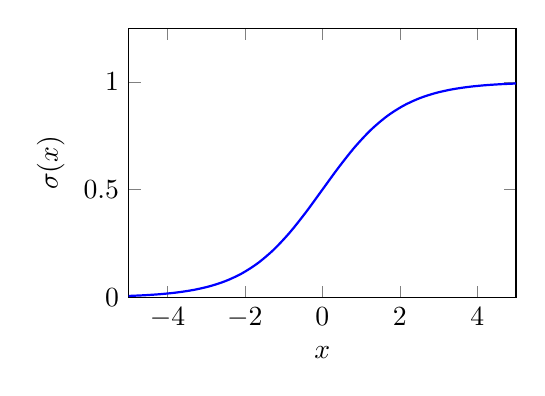
\begin{tikzpicture}
			\begin{axis}[width=6.5cm,height=5cm,ylabel=$\sigma(x)$,xlabel=$x$,ymin=0,ymax=1.25,xmin=-5,xmax=5]
				\addplot[thick,blue,smooth] {1/(1+exp(-x))};
			\end{axis}
		\end{tikzpicture}
	}
	\subfigure[hyperbolic tangent ($\tanh$)]{
		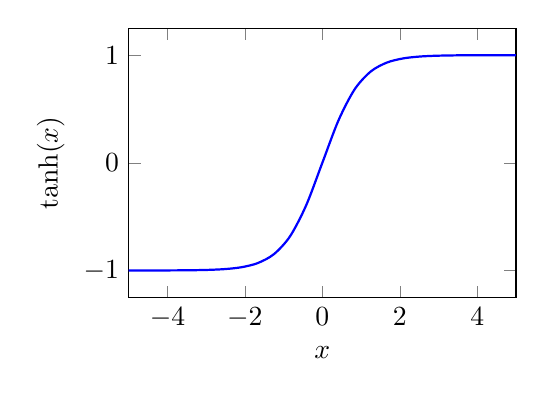
\begin{tikzpicture}
			\begin{axis}[width=6.5cm,height=5cm,ylabel=$\tanh(x)$,xlabel=$x$,ymin=-1.25,ymax=1.25,xmin=-5,xmax=5]
				\addplot[thick,blue,smooth] {tanh(x)};
			\end{axis}
		\end{tikzpicture}
	}\\
	\subfigure[rectified linear unit ($\operatorname{ReLU}$))]{
    		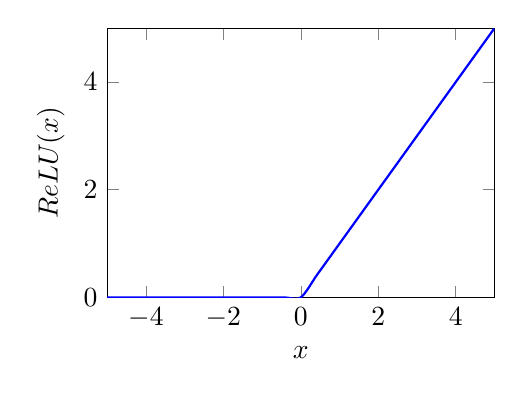
\begin{tikzpicture}
			\begin{axis}[width=6.5cm,height=5cm,ylabel=$\operatorname{ReLU}(x)$,xlabel=$x$,ymin=0,ymax=5,xmin=-5,xmax=5]
				\addplot[thick,blue,smooth] {max(0, x)};
			\end{axis}
		\end{tikzpicture}
	}
	\subfigure[Heaviside step function ($s$)]{
		\begin{tikzpicture}
			\begin{axis}[width=6.5cm,height=5cm,ylabel=$\operatorname{s}(x)$,xlabel=$x$,ymin=0,ymax=1.25,xmin=-5,xmax=5]
                \addplot[thick,blue,mark=*,samples at={-100,0}] {0};
                \addplot[thick,blue,mark=*,mark options={fill=white},samples at={0,100}] {1};
			\end{axis}
		\end{tikzpicture}
	}
    	\caption[Commonly used activation functions.]{Commonly used activation functions }
    	\label{fig:introduction:dl:activation-fns}
\end{figure}
\newpage